\documentclass[conference]{IEEEtran}

\usepackage{cite}
\usepackage{amsmath}
\usepackage{booktabs}
\usepackage{balance}
\usepackage{graphicx}
\usepackage{siunitx}
\usepackage{xcolor}
\usepackage[section]{placeins}
\usepackage{tikz}
\usepackage{pgfplots}
\usepackage{pgfplotstable}
\usepackage[caption=false,font=footnotesize]{subfig}
\usepackage[hidelinks]{hyperref}

\pgfplotsset{compat=1.18}
\usepgfplotslibrary{groupplots}
\sisetup{
  round-mode=places,
  round-precision=3,
  detect-all
}

\definecolor{coreblue}{HTML}{1F77B4}
\definecolor{socred}{HTML}{D62728}
\definecolor{fpgaorange}{HTML}{FF7F0E}
\definecolor{simgreen}{HTML}{2CA02C}
\definecolor{softgray}{HTML}{666666}

\title{Prometheus SoC: High-Level Synthesis of a RISC-V Softmax Accelerator System on the PYNQ-Z1}

\author{
\IEEEauthorblockN{Jesse Levine}
\IEEEauthorblockA{
Department of Electronics\\
Carleton University\\
Ottawa, Canada
}
}

\begin{document}
\maketitle

\begin{abstract}
This paper consolidates a multi-phase hardware design study into a single research narrative centered on Softmax acceleration for resource-constrained edge systems. Starting from a reproduced high-level synthesis (HLS) RV32I RISC-V processor, the work first extends the core to RV32IM, then optimizes the baseline through pipelining, and finally integrates a dedicated fixed-point Softmax accelerator into a shared-memory system-on-chip (SoC) called \emph{Prometheus SoC}. The accelerator uses max-subtraction for numerical stabilization, piecewise-linear exponential and reciprocal approximations, and a four-lane vectorized datapath implemented with HLS dataflow. The resulting system is exposed to the processor through memory-mapped I/O and deployed on a Digilent PYNQ-Z1. Across the implementation-level comparison used for architecture selection, the software-only core scales as $287.89N + 74.34$ cycles, while the integrated SoC scales as $0.74N + 226.61$ cycles. This yields a measured speedup of $114.7\times$ at $N=128$ and an asymptotic slope-based limit of approximately $389\times$. The accelerator also restores Softmax normalization accuracy, maintaining sums near unity while the software baseline degrades substantially with increasing vector length. FPGA measurements from the implemented SoC match simulation exactly at the sampled verification points and meet timing at \SI{84.2}{\mega\hertz}. Together, these results justify the final architectural choice of a tightly integrated RISC-V plus accelerator SoC.
\end{abstract}

\begin{IEEEkeywords}
RISC-V, high-level synthesis, FPGA, Softmax, hardware accelerator, PYNQ-Z1, SoC
\end{IEEEkeywords}

\section{Introduction}
Softmax is a small kernel in source-code size, but it is a disproportionately expensive kernel in hardware-constrained inference systems. Its computation requires exponentiation, accumulation, and normalization over an entire vector:
\begin{equation}
\sigma(z)_i = \frac{e^{z_i}}{\sum_{j=1}^{N} e^{z_j}}.
\end{equation}
On a small integer-oriented processor, these operations are instruction-bound and numerically fragile when implemented through fixed-point software approximations. At the same time, Softmax remains architecturally relevant because it is the final normalization step in classifiers and a core operation inside Transformer attention pipelines \cite{vaswani2017attention}.

This project began from the HLS RV32I SoC of Toker \cite{toker2023hlsriscv}, then evolved toward a specialized accelerator informed by recent approximation-based Softmax hardware for Transformer workloads \cite{kim2025softmax}. The final result is not a standalone accelerator, but a complete RISC-V plus accelerator SoC that preserves processor control while offloading the numerically intensive Softmax path into dedicated hardware.

The main contributions of this work are:
\begin{enumerate}
\item a consolidated hardware progression from baseline RV32I reproduction to an RV32IM, pipelined, Softmax-capable system;
\item a fixed-point Softmax accelerator with log-sum-exp stabilization, piecewise-linear exponential and reciprocal approximations, and a four-lane vectorized datapath;
\item a shared-BRAM, MMIO-controlled SoC integration that allows a RISC-V core to launch and read back accelerator results without DMA; and
\item end-to-end validation on the PYNQ-Z1, including architecture-selection plots, board-level implementation data, and FPGA-versus-simulation agreement.
\end{enumerate}

\section{Related Work}
Toker \cite{toker2023hlsriscv} demonstrates that a compact RV32I-based SoC can be described and implemented through HLS, providing the methodological starting point for this project. That work is important here because it shows that a soft RISC-V processor can be treated as a synthesizable HLS design object rather than only as handcrafted RTL. The first phase of this project reproduced that baseline and verified its fetch-decode-execute behavior on FPGA.

Kim \emph{et al.} \cite{kim2025softmax} focus instead on the non-linear bottlenecks of Transformer inference and show that approximation-based Softmax and LayerNorm acceleration can achieve strong speedups with controlled accuracy loss. Their work motivates the use of piecewise-linear approximation for the exponential and fixed-point-friendly normalization paths. The present paper differs in scope and target: instead of accelerating large Transformer layers on a high-end FPGA, it integrates a Softmax-specific accelerator into a small HLS RISC-V SoC on a Zynq-7020-class board.

The position of this work is therefore between those references. It begins from an HLS RISC-V system in the style of \cite{toker2023hlsriscv}, then specializes that system around the Softmax bottleneck highlighted by \cite{kim2025softmax}, while keeping the processor in the loop as the software controller.

\section{Project Evolution and Final Architecture}
The project evolved through five reports that directly informed the final system. Report~1 reproduced the RV32I baseline and established the bare-metal memory-image workflow. Report~2 extended the baseline to RV32IM so multiplication-based fixed-point kernels became practical. Report~3 proposed the specialization strategy: approximate exponentiation, memory-mapped control, and shared memory between processor and accelerator. Report~5 delivered the first pipelined RV32IM baseline and a standalone Softmax accelerator. Report~6 integrated these ideas into the final \emph{Prometheus SoC}, which is the focus of this paper.

\begin{figure}[t]
\centering
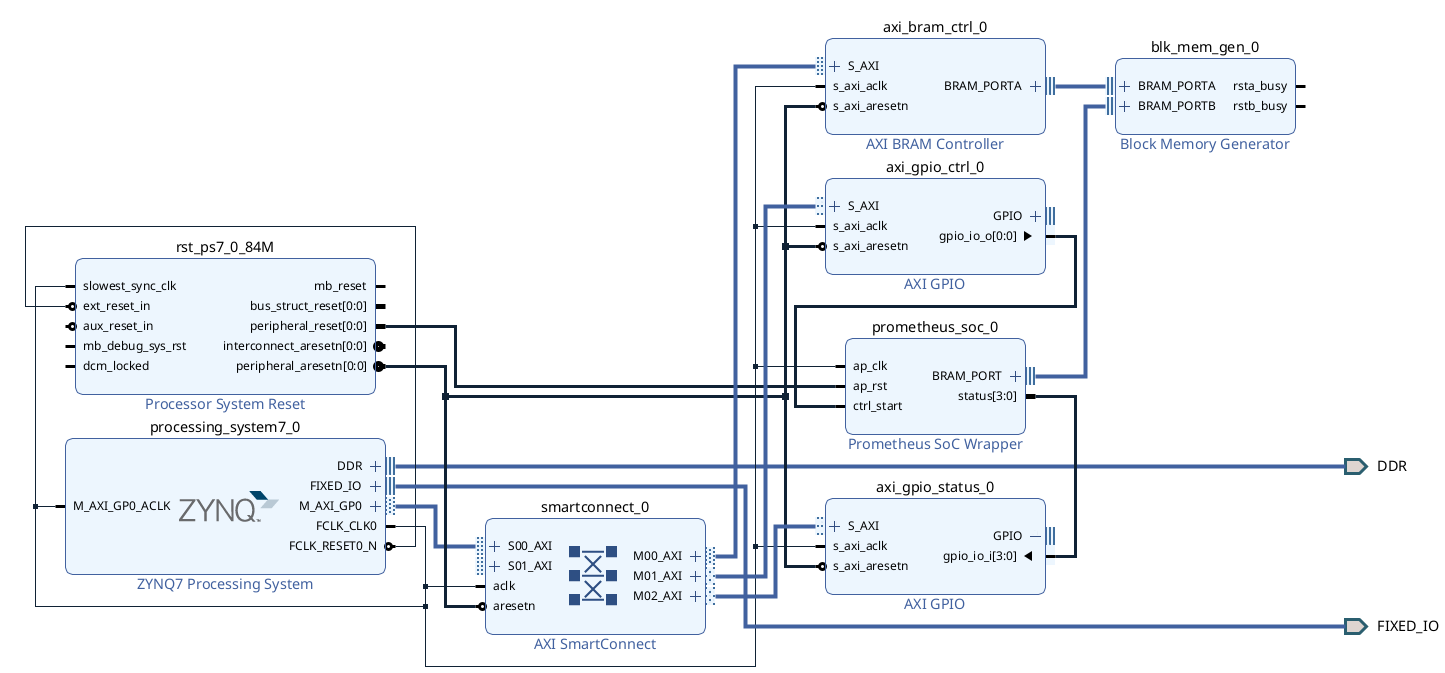
\includegraphics[width=\columnwidth]{figures/report6-000.png}
\caption{Vivado block diagram of the implemented Prometheus SoC on the PYNQ-Z1. The Zynq processing system provides AXI control, while the programmable logic contains the packaged Prometheus SoC wrapper, AXI BRAM controller, shared BRAM, and GPIO-based start/status path.}
\label{fig:block_diagram}
\end{figure}

Fig.~\ref{fig:block_diagram} shows the final deployed system. The Zynq processing system acts as host-side control logic and accesses the programmable logic through AXI SmartConnect. Shared BRAM holds the RISC-V program image, input logits, output probabilities, and debug words. Two AXI GPIO blocks implement a simple hardware-software handshake: one pulses the start signal, and the other returns latched status bits and FPGA cycle counts.

Inside the packaged HLS core, the RISC-V processor and accelerator share the same memory image. The software configures the accelerator through MMIO registers at address \texttt{0x7000}, writing the input base address, output base address, debug base address, and vector length $N$, then setting the start bit. The accelerator reads logits from BRAM, computes exponentials after subtracting the vector maximum, accumulates the sum, computes an approximate reciprocal, and writes normalized probabilities back into BRAM. This integration avoids explicit data copying and keeps the processor responsible for orchestration rather than numerical throughput.

The exponential path exploits the identity
\begin{equation}
e^x = 2^{x / \ln 2},
\end{equation}
implemented with a fixed-point multiply by $1 / \ln 2$, a power-of-two shift for the integer component, and a 17-point piecewise-linear lookup for the fractional component. The final accelerator version uses a four-word vector width and HLS dataflow so memory movement and arithmetic can overlap.

Measured across the project reports, the architecture progression is consistent: each stage traded additional area for a lower marginal Softmax cost. The important qualitative transition was from software execution on the pipelined core, to a standalone accelerator, and finally to an integrated SoC in which the processor remains the controller while the accelerator handles the numerically intensive kernel.

\section{Experimental Methodology}
The evaluation combines data from the implementation-level comparisons used during architecture selection and the board-level FPGA validation performed on the final system. The software baseline is the pipelined RV32IM core from Report~5. The final system is the integrated Prometheus SoC deployed on the Digilent PYNQ-Z1 with the \texttt{xc7z020clg400-1} device.

All Softmax inputs use fixed-point Q16.16 values. For the architecture-selection study, vector lengths from $N=2$ to $N=128$ are compared using the same workload set previously reported for the core-only and SoC implementations. For board validation, the SoC is swept from $N=2$ to $N=256$ through the JTAG/PYNQ execution flows stored in the repository, and the resulting FPGA cycle counts and normalization sums are recorded. The primary metrics are:
\begin{itemize}
\item clock cycles versus sequence length;
\item Softmax probability sum as a numerical-stability proxy;
\item implementation resource cost; and
\item simulation-versus-FPGA agreement for the final SoC.
\end{itemize}

\section{Results}
\subsection{Implementation-Level Architecture Selection}
\begin{table}[t]
\centering
\caption{Implementation-level resource summary used for architecture selection. The baseline values come from the pipelined RV32IM implementation flow, while the SoC values come from the Prometheus SoC Vivado IP-flow implementation.}
\label{tab:impl_compare}
\begin{tabular}{lcc}
\toprule
Resource / Metric & Core Only & Core + Accelerator SoC \\
\midrule
LUT & 2169 & 26090 \\
FF & 1465 & 52339 \\
DSP & 12 & 32 \\
BRAM & 0 & 9 \\
Post-route period (ns) & 11.345 & 11.514 \\
\bottomrule
\end{tabular}
\end{table}

Table~\ref{tab:impl_compare} captures the central design trade-off. The integrated SoC is substantially larger than the software-only baseline because it includes the accelerator datapath, extra local buffering, and the MMIO-based control structure. The architectural question is therefore whether this area increase is justified by the system-level throughput and accuracy gains.

\begin{figure}[!t]
\centering
\begin{tikzpicture}
\begin{groupplot}[
    group style={group size=1 by 2, vertical sep=1.0cm},
    width=0.43\textwidth,
    height=3.5cm,
    xlabel={Sequence length $N$},
    grid=both,
    grid style={gray!20},
    tick label style={font=\small},
    label style={font=\small}
]
\nextgroupplot[ylabel={Core cycles}]
\addplot+[black, mark=*, thick] table[x=n,y=core_cycles,col sep=comma] {data/core_vs_soc.csv};
\nextgroupplot[ylabel={SoC cycles}]
\addplot+[black, mark=square*, thick] table[x=n,y=soc_cycles_sim,col sep=comma] {data/core_vs_soc.csv};
\end{groupplot}
\end{tikzpicture}
\caption{Latency scaling of the software-only core and the integrated SoC on separate axes. A shared axis hides the SoC behavior because the software baseline is so much slower.}
\label{fig:latency_compare}
\end{figure}

\begin{figure}[!t]
\centering
\begin{tikzpicture}
\begin{axis}[
    width=0.46\textwidth,
    height=4.4cm,
    xlabel={Sequence length $N$},
    ylabel={Softmax sum},
    ymin=0.64,
    ymax=1.02,
    grid=both,
    grid style={gray!20},
    legend style={at={(0.03,0.97)}, anchor=north west, draw=none, fill=none, font=\small},
    tick label style={font=\small},
    label style={font=\small}
]
\addplot+[color=coreblue, only marks, mark=*, mark size=1.8pt] table[x=n,y=core_sum,col sep=comma] {data/core_vs_soc.csv};
\addlegendentry{Core only}
\addplot+[color=socred, only marks, mark=square*, mark size=1.8pt] table[x=n,y=soc_sum_sim,col sep=comma] {data/core_vs_soc.csv};
\addlegendentry{Core + accelerator}
\addplot[dashed, color=softgray] coordinates {(0,1) (140,1)};
\end{axis}
\end{tikzpicture}
\caption{Normalization comparison between the software-only core and the integrated SoC. The software path loses probability mass as $N$ grows, while the accelerator maintains sums close to unity.}
\label{fig:sum_compare}
\end{figure}

Fig.~\ref{fig:latency_compare} shows the throughput result that motivated the final architecture choice: the software-only baseline scales linearly but with a very large slope, while the integrated SoC keeps the per-element cost extremely small. Fig.~\ref{fig:sum_compare} explains the corresponding numerical result. The software-only core does not merely run slower; its fixed-point approximation path causes the Softmax sum to collapse toward approximately $0.675$ for longer vectors, which indicates significant accumulated numerical error. In contrast, the accelerator maintains sums close to $1.0$ across the tested range because it uses explicit max-subtraction and a dedicated normalization path rather than long software sequences for exponentiation and reciprocal evaluation. This is the first result that makes the final architecture selection credible: the accelerator is not only faster, it is materially better behaved numerically.

\begin{figure}[!t]
\centering
\begin{tikzpicture}
\begin{axis}[
    width=0.46\textwidth,
    height=4.5cm,
    xlabel={Sequence length $N$},
    ylabel={Speedup ratio},
    ymin=0,
    ymax=125,
    grid=both,
    grid style={gray!20},
    tick label style={font=\small},
    label style={font=\small}
]
\addplot+[black, mark=triangle*, thick] table[x=n,y=speedup,col sep=comma] {data/core_vs_soc.csv};
\end{axis}
\end{tikzpicture}
\caption{Measured speedup of the integrated SoC over the software-only core. The slope ratio from the earlier implementation study implies an asymptotic upper bound of approximately $389\times$.}
\label{fig:speedup_compare}
\end{figure}

Fig.~\ref{fig:speedup_compare} shows that speedup grows rapidly with vector length because both systems scale linearly but with very different slopes. The measured ratio exceeds $114\times$ at $N=128$. Using the previously reported trend lines, the theoretical large-$N$ speedup limit is approximately $287.89 / 0.74 \approx 389\times$. This asymptotic framing is useful because it explains why the SoC overhead at small $N$ does not change the long-range architectural conclusion.

\subsection{PYNQ-Z1 FPGA Implementation}
\begin{table}[t]
\centering
\caption{Implemented PYNQ-Z1 summary for the full Prometheus SoC. This table refers to the complete board-integrated design rather than only the packaged HLS IP block.}
\label{tab:fpga_soc}
\begin{tabular}{lc}
\toprule
Metric & Implemented SoC on PYNQ-Z1 \\
\midrule
Board & Digilent PYNQ-Z1 \\
FPGA & \texttt{xc7z020clg400-1} \\
Clock period (ns) & 11.875 \\
Clock frequency (MHz) & 84.211 \\
WNS (ns) & 0.332 \\
WHS (ns) & 0.010 \\
Slice LUTs & 32717 \\
Slice Registers & 60358 \\
Block RAM Tiles & 68.5 \\
DSPs & 32 \\
Timing status & Met \\
\bottomrule
\end{tabular}
\end{table}

Table~\ref{tab:fpga_soc} shows that the full board-level design closed timing on the target FPGA. This matters because the final deliverable is not a simulation-only argument. The processor, shared BRAM, AXI glue logic, GPIO path, and accelerator were implemented together in a deployable system and exercised on hardware.

\begin{figure}[!t]
\centering
\subfloat[FPGA latency sweep.]{
\begin{tikzpicture}
\begin{axis}[
    width=0.46\textwidth,
    height=3.6cm,
    xlabel={Sequence length $N$},
    ylabel={Clock cycles},
    grid=both,
    grid style={gray!20},
    tick label style={font=\small},
    label style={font=\small}
]
\addplot+[black, mark=*, thick] table[x=n,y=cycles,col sep=comma] {data/prometheus_soc_n_sweep.csv};
\end{axis}
\end{tikzpicture}
}

\vspace{2mm}

\subfloat[FPGA normalization behavior.]{
\begin{tikzpicture}
\begin{axis}[
    width=0.46\textwidth,
    height=3.6cm,
    xlabel={Sequence length $N$},
    ylabel={Softmax sum},
    ymin=0.9975,
    ymax=1.001,
    ytick={0.998,0.999,1.000,1.001},
    yticklabel style={/pgf/number format/fixed,/pgf/number format/precision=4},
    grid=both,
    grid style={gray!20},
    tick label style={font=\small},
    label style={font=\small}
]
\addplot+[black, only marks, mark=*, mark size=1.5pt] table[x=n,y=sum,col sep=comma] {data/prometheus_soc_n_sweep.csv};
\addplot[dashed, color=softgray] coordinates {(0,1) (260,1)};
\end{axis}
\end{tikzpicture}
}
\caption{Measured FPGA behavior of the implemented Prometheus SoC across the full sweep.}
\label{fig:fpga_validation}
\end{figure}

Fig.~\ref{fig:fpga_validation} confirms that the FPGA implementation preserves the intended system behavior across the full tested range. Latency remains low and grows gently with $N$, while the Softmax sum stays close to $1.0$. Even at $N=256$, the measured sum remains $0.997955$, which is consistent with fixed-point quantization rather than an architectural failure.

The strongest end-to-end validation result is the simulation-versus-FPGA agreement at representative points. At $N=\{2,8,32,64,128\}$, the FPGA cycle counts match the simulated cycle counts exactly: $229$, $232$, $250$, $274$, and $322$ cycles, respectively. The normalization sums also match to the printed precision, with the corresponding FPGA latencies ranging from \SI{2.719}{\micro\second} at $N=2$ to \SI{3.824}{\micro\second} at $N=128$. This validates not only the accelerator arithmetic, but also the correctness of the MMIO control path, shared-memory addressing, and integration wrapper.

\section{Discussion}
The combined evidence supports a clear architectural conclusion. A software-only implementation on a small RISC-V core is not an attractive endpoint for Softmax-heavy workloads because its per-element cost is too high and its fixed-point approximation path degrades normalization quality as vectors grow. The standalone accelerator already resolves most of the throughput problem, but the integrated SoC is the more useful system architecture because it preserves software programmability and embeds the accelerator in the same memory space as the processor.

The main limitation of the present design is scope rather than correctness. The integrated system accelerates Softmax only; it does not yet offload the earlier matrix-heavy layers of a full neural network, and it uses fixed-point arithmetic tuned for the tested workloads rather than a broad accuracy study over large benchmark suites. These are reasonable future directions. Another useful next step would be extending the accelerator interface beyond the current BRAM-centric deployment to a larger memory subsystem or DMA-capable integration.

\section{Conclusion}
This paper consolidated the full project progression from a reproduced HLS RV32I core to a deployed RISC-V plus accelerator SoC. The final architecture, Prometheus SoC, integrates a four-lane fixed-point Softmax accelerator with a RISC-V controller through shared BRAM and MMIO. Relative to the software-only pipelined RV32IM baseline, the integrated system reduces the effective marginal Softmax cost from $287.89$ cycles per element to $0.74$ cycles per element, delivers a measured $114.7\times$ speedup at $N=128$, preserves normalization accuracy near unity, and matches simulation when exercised on the PYNQ-Z1 FPGA. These results make the final architecture selection straightforward: the publishable contribution is not only an accelerator, but a validated SoC-level demonstration of hardware-software co-design for Softmax acceleration on a constrained FPGA platform.

\appendices
\section{Summary of AI Usage}
AI tools were used throughout the project as engineering assistants rather than as sources of experimental results. In the early phases, they were used to help interpret the reference RV32I architecture, understand HLS reports, and construct the bare-metal software flow used to generate memory-image test programs. During the accelerator and SoC phases, they were used to accelerate implementation work such as code drafting, testbench construction, script development, and explanation of synthesis and FPGA integration artifacts.

For this final paper, AI assistance was used to consolidate the prior reports into a single narrative, recover and cross-check stored datasets, generate and refine the \LaTeX{} manuscript structure, and review consistency between the paper claims and the repository implementation. AI was also used after the paper was completed to derive a spoken presentation script from the manuscript and to generate a narrated audio version through a text-to-speech API so that the project could be presented in an audio format. That presentation workflow affected only dissemination artifacts and did not contribute any experimental data, measurements, or technical claims to the paper itself.

All architectural claims, numerical values, figures, and tables in the final manuscript were checked against the project source files, build artifacts, and measured outputs before inclusion.

\FloatBarrier
\balance

\begin{thebibliography}{00}

\bibitem{vaswani2017attention}
A.~Vaswani, N.~Shazeer, N.~Parmar, J.~Uszkoreit, L.~Jones, A.~N. Gomez,
L.~Kaiser, and I.~Polosukhin, ``Attention is all you need,'' in \emph{Advances in Neural Information Processing Systems}, vol.~30, 2017.

\bibitem{toker2023hlsriscv}
O.~Toker, ``A high-level synthesis approach for a RISC-V RV32I-based system on chip and its FPGA implementation,'' \emph{Engineering Proceedings}, vol.~58, no.~1, p.~72, 2023, doi: \href{https://doi.org/10.3390/ecsa-10-16212}{10.3390/ecsa-10-16212}.

\bibitem{kim2025softmax}
R.~Kim, D.~Lee, J.~Kim, J.~Park, and S.~E. Lee, ``Hardware accelerator for approximation-based softmax and layer normalization in transformers,'' \emph{Electronics}, vol.~14, no.~12, p.~2337, 2025, doi: \href{https://doi.org/10.3390/electronics14122337}{10.3390/electronics14122337}.

\bibitem{riscvmanual}
A.~Waterman and K.~Asanovi\'c, Eds., \emph{The RISC-V Instruction Set Manual, Volume I: Unprivileged ISA}, document version 20191214, RISC-V Foundation, 2019.

\end{thebibliography}

\end{document}
